\chapter[SM SysId of LTI systems with EIV noise structure]{Set-Membership SysId of LTI systems with Errors-In-Variables (EIV) noise structure}

We have seen in the last chapter that an equation-error noise structure leads to a solution of LP problems for obtaining the Parameter Uncertainty Intervals, however, we have seen that there are some drawbacks. 
First of all the way we can find a bound $\Delta_e$ on the noise samples.
Then, the objective here is to find a way for dealing with the 'original' problem, that is the one using the output and input samples corrupted by noise. In order to gradually present all the needed ingredients for properly solving the problem, we show in turn general teoretical results and examples in which such results are applied to our problem of \textit{System Identification}.

\section{ Feasible Parameter Set in the EIV set-up}
In order to define also for this type of set-up the feasible parameter set, we have to follow the same road as we have done before. In particular we have to put together:
\begin{description}
    \itemsep-0.2em
    \item[A-priori information on the system] We know that the system belongs to a certain class $\mathcal{F}$, moreover we know the order $n$ of the system itself.
    \item[A-priori information on the noise] In particular the way the uncertainty enters the identification problem (we assume here the most general case when both input and output are corrupted by noise) and the boundedness of the noise samples, in particular
    \begin{equation}
        \vert \eta(k) \vert \le \Delta_\eta \quad
        \vert \xi(k) \vert \le \Delta_\xi
        \quad
        \forall k=1,...,N
    \end{equation}
    \item[A-posteriori information] They are nothing but the experimentally collected data $$\tilde{y}(k)=y(k)+\eta(k), \quad 
    \tilde{u}(k)=u(k)+\xi(k) $$
\end{description}
For an \textbf{LTI system of order $n$} the feasible parameter set is defined as follows: 

\begin{equation}\label{eq:FPS}
    \begin{aligned}
        \mathcal{D}_\theta = \{
            &\theta\in\mathbb{R}^p:  
            (\tilde{y}(k)-\eta(k))+\sum_{i=1}^n{\theta_i}\ ({y}(k-i)-\eta(k-i))=\\
            &\sum_{j=0}^m \theta_j \ (u(k-j)-\xi(k-j)), \quad
            k=n+1,...,N
        \} 
    \end{aligned}
\end{equation}
\noindent
In this context the definition of PUI is always the same, and the extrema of such an interval are defined as before by  solving the optimization problems:

\begin{equation*}
    \underline{\theta}_j = \min_{\theta\in\mathcal{D}_\theta} \theta_j, \quad 
    \overline{\theta}_j = \max_{\theta\in\mathcal{D}_\theta} \theta_j
    \Longrightarrow PUI_{\theta_j}=[\underline{\theta}_j,\overline{\theta}_j]
\end{equation*}
At this point the question is: \textbf{what type of $\mathcal{D}_\theta$ I obtain?} 
\section{Extended Feasible Parameter Set $\mathcal{D}_{\theta,\eta,\xi}$}
How we are able to see in the (\ref{eq:FPS}) the set definition depends also on the noise samples. The difference here is that I cannot eliminate them without adding any approximation. Substancially, I am introducing a non trivial number of new unknown in the description of the set: for $N$ collected samples, $2N$ new variables are added, which cannot be eliminated. For this reason we have to \textit{enlarge} the set $\mathcal{D}_\theta$ involving also the new variables. In this way we introduce the so-called \textbf{Extended Feasible Parameter Set (EFPS)} which we indicate with $\mathcal{D}_{\theta,\eta,\xi}$. \\
In order to better understand this aspect, let us consider a toy-example in which we have a single parameter $\eta(1)$ which is added to the pair $\theta_1, \theta_2$. The EFPS in this case -- how the figure below shows -- is a subset of $\mathbb{R}^3$.
\vspace{-0.2cm}
\begin{figure}[h]
    \centering
    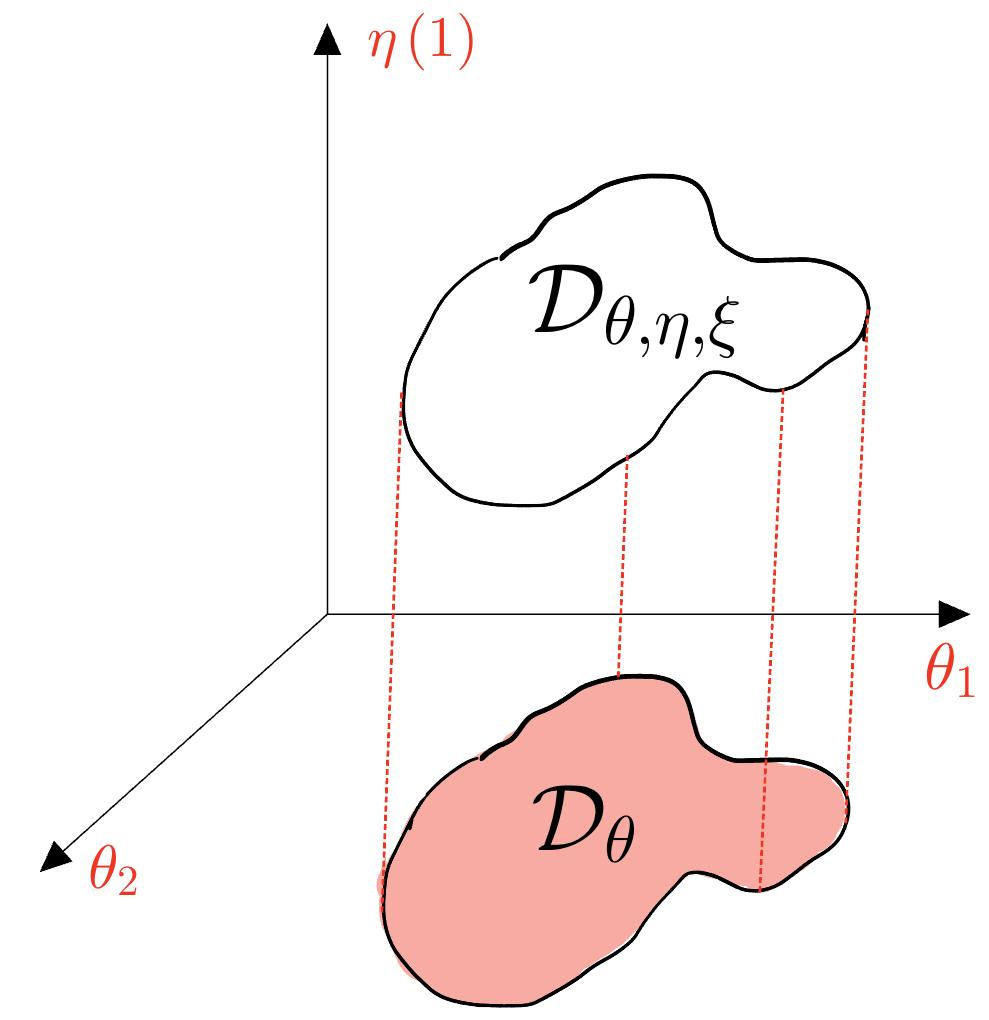
\includegraphics[scale=0.15]{img/EFPS.jpeg}
    \caption{Example in $\mathbb{R}^3$ of the Extended feasible parameter set}
\end{figure}

\noindent
The FPS $\mathcal{D}_\theta$ is nothing but the projection on the $(\theta_1,\theta_2)$ plane of the set $\mathcal{D}_{\theta,\eta}$, in this case no parameter $\xi$ is present.

\noindent
The definition of the \textbf{Extended Feasible Parameter Set} becomes the following:
\begin{equation}
    \begin{aligned}
        \mathcal{D}_{\theta,\eta,\xi} = \{
            &\theta\in\mathbb{R}^p, \eta\in\mathbb{R}^N, \xi \in \mathbb{R}^N: 
            \tilde{y}(k)-\eta(k) + \theta_1 (y(k-1)-\eta(k-1)) +\\
            &+\theta_2 (y(k-2)-\eta(k-2))+\dots+\theta_n (y(k-n)-\eta(k-n))=\\
            &=\theta_{n+1} (u(k)-\xi(k))+\theta_{n+2} (u(k-1)-\xi(k-1)) + ...+\\
            &\theta_{n+m+1} (u(k-m)-\xi(k-m)), \quad k=n+1,...,N\\
             &\vert \xi(k) \vert \le \Delta_\xi, \quad 
            \vert \eta(k) \vert \le \Delta_\eta, \quad k=1,...,N
        \}
    \end{aligned}
\end{equation}

\noindent
Such a set is defined by \textbf{nonlinear} and \textbf{non-convex} constraints and then the set is non-convex. In the specific case, the constraints that arises are \textbf{bilinear ones} which are a particular class of \textbf{polynomial constraints}. In general we know that is very hard to obtain a global minimum from a non-convex optimization problem, in this case using some tools for \textit{polynomial optimization} it is possible to reach a global minimum.\\

\noindent
In this framework the problem of finding the PUIs becomes:
{\large{
    \begin{equation}\label{eq:PUI_delta}
        PUI_{\theta_j} = [\underline{\theta}_j,\overline{\theta}_j] \Longrightarrow 
        \underline{\theta}_j = \min_{\theta\in\mathcal{D}_{\theta,\eta,\xi} } \theta_j,    \quad
        \overline{\theta}_j = \max_{\theta\in\mathcal{D}_{\theta,\eta,\xi}} \theta_j
    \end{equation}
}}

\section{Convex relaxation for Polynomial Optimization Problems (POPs)}
\begin{center}
    \textsf{
    In this section we will introduce some general theoretical results on polynomial optimization problems, that -- how we have seen -- are the ones arising in the definition of the extended feasible parameter set (EFPS). We will start by formulating them, we will analyze the type of sets they produce and finally we will introduce the concept of \textbf{convex relaxation}.}
\end{center}

\noindent 
Let us consider the following general optimization problem:
\begin{equation}
    \begin{aligned}
        \min_{x} &f_0(x)\\ 
        &\text{s.t.} \ f_k(x)\le{0} \quad k=1, ..., l\\
        &f_k(x)=0 \quad k=l+1,...,m
    \end{aligned}
\end{equation}
where $f_0$ and $f_k, \ k=1,...,m$ are \textbf{multivariate polynomials} in the optimization variable $x$. Giving an example if $x=[x_1\ x_2\ x_3]^T$, an example of $f_0$ is
\begin{equation*}
    f_0(x)=x_1^2+x_2{x_3^3}+x_1^5{x_2^3}+7{x_3^2}
\end{equation*}
All POPs can be written, for sure, in the so-called \textbf{epigraphic form} by introducing a scalar (slack) variable $\gamma$.

\begin{multicols}{2}
    \noindent
    \textbf{\color{red}Original formulation}
    \begin{equation}
        \begin{aligned}
            \min_{x\in\mathbb{R}^n} &\ f_0(x)\\ 
            &\text{s.t.} \ f_k(x)\le{0} \quad k=1, ..., l\\
            &f_k(x)=0 \quad k=l+1,...,m
        \end{aligned}
    \end{equation}
    \newcolumn\\
    \textbf{\color{red}Epigraphic formulation}
    \begin{equation}
        \begin{aligned}
            \min_{x\in\mathbb{R}^n, \gamma \in \mathbb{R}} &\ \gamma\\ 
            &\text{s.t.} \ f_0(x)\le\gamma\\
            &f_k(x)\le{0} \quad k=1, ..., l\\
            &f_k(x)=0 \quad k=l+1,...,m
        \end{aligned}
    \end{equation}
\end{multicols}
\noindent
By rewriting a generic POP in the epigraphic form, it becomes a problem of \textbf{minimizing a linear function over a non-convex set described by polynomial constraints} (this is also true  for the unconstrained case).

\begin{figure}[h] \label{fig:non-convex}
    \centering
    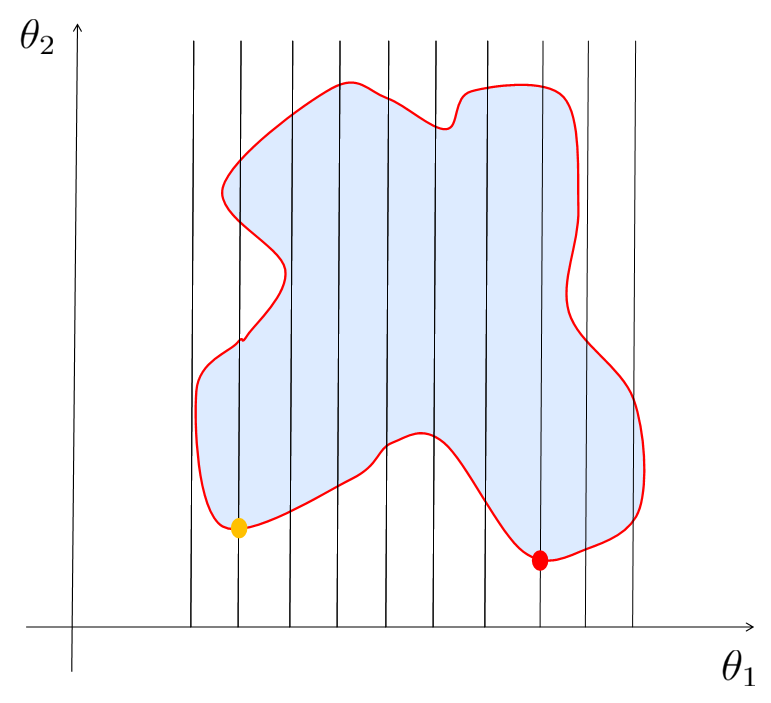
\includegraphics[scale=0.5]{img/nonconvex.png}
    \caption{Example of min a linear objective (thin line) over a non-convex set (sky-blue)}
\end{figure}

The figure (\ref{fig:non-convex}) shows the general idea. We are moving a linear objective (thin lines in black) over the set in sky-blue derived by the polynomial (so non-convex) constraints. The thin lines are the so-called \textit{level-curves} in order to minimize $\theta_1$. Moreover the orange point is a \textbf{local minimum}, while the red one is the \textbf{global minimum}.\\

\noindent
\textbf{\color{red}Important remark:} since a generic POP can written in epigrapigh form, we can note that the non-convexity of  the problem is now \textbf{completely embedded} in the description of the set of constraints $\to$ whether we want to compute the \textbf{global optimal solution} we have to deal with the non-convexity of the set of constraints. It is very high the probability of getting stuck in local minima.\\

\begin{definition}[Convex hull of a non-convex set] Given a non-convex set $\mathcal{S}$, the \textbf{convex hull} for it is the smallest  convex-set including $\mathcal{S}$. 
\end{definition}

A very-nice property is that the \textbf{min/max} computed on the convex hull is equal to the one computed on the original set. In this way we gain the convexity of the problem. 

In other words,if we are able to write down the equations describing the convex hull $C_\mathcal{S}$ of the non-convex set $\mathcal{S}$ we have that:
\begin{equation}
    \min_{x\in{C_\mathcal{S}}} f(x) = \min_{x\in\mathcal{S}} f(x)
\end{equation}
The drawback here is that, in general, obtaining a mathematical description of $C_\mathcal{S}$ is a quite difficult problem.\\
In the particular case of POPs, it is possible to compute a \textbf{convex relaxation os $\mathcal{S}$} depending on a parameter called the \textbf{order of relaxation} $\delta$.

\begin{figure}[h]
    \centering
    \subfigure[Convex hull $C_\mathcal{S}$]{
        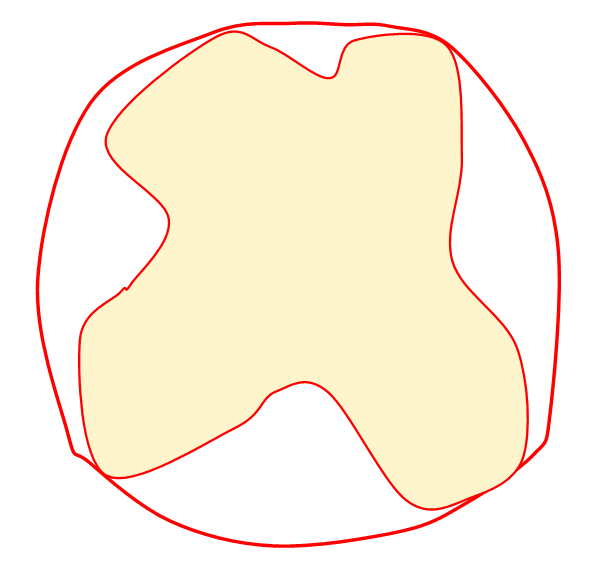
\includegraphics[scale=0.5]{img/convex_hul..png}
    }
    \subfigure[Relaxing the convex hull by $\delta$]{
        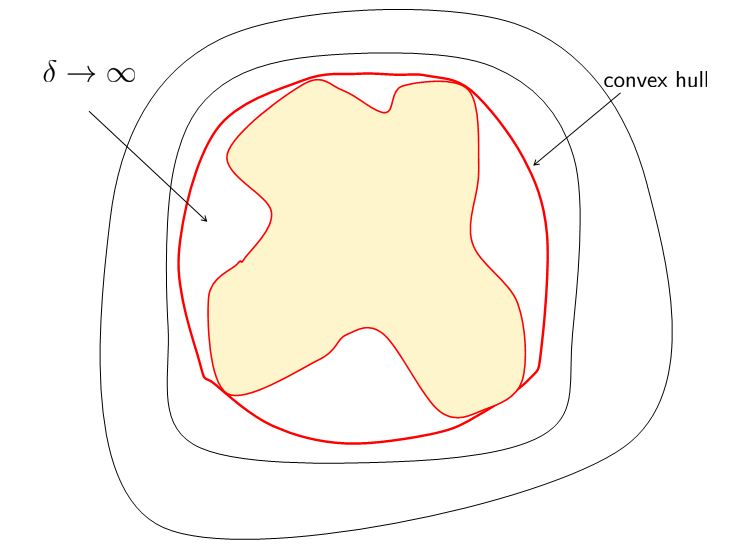
\includegraphics[scale=0.5]{img/relax.png}
    }
\end{figure}
\begin{figure}[h]
    \centering    
\end{figure}

For a given $\delta$ we have different relaxed sets as you can see in the figure, moreover for $\delta\to\infty$ the relaxed set coincides with the convex hull in red.\\
All of this concepts are then applied to our optimization problem which is aimed to find the extrema of the Parameter Uncertainty Intervals for our problem of System Identification. In this case comes up an interesting property, that is, for sure whatever is the order $\delta$, we are including the real PUI. More specifically, we have that for each $k$ the relaxed solutions $\underline{\theta}_k^{\delta}$ and $\overline{\theta}_k^{\delta}$ are such that:
{\large{
    \begin{equation}
        \underline{\theta}_k^{\delta} \le \underline{\theta}_k
        \quad 
        \overline{\theta}_k^{\delta} \le \overline{\theta}_k
    \end{equation}
}}
moreover it holds that: 
\begin{equation}
    \lim_{\delta\to\infty} \underline{\theta}_k^{\delta} = \underline{\theta}_k \quad
    \lim_{\delta\to\infty} \overline{\theta}_k^{\delta} = \overline{\theta}_k
\end{equation}

\noindent
In order to solve a POP by means of \textit{Lassere convex  relaxation approach} in MATLAB we use:
\begin{enumerate}
    \item \textsf{SparsePOP} that given a polynomial optimization problem and the order of relaxation $\delta$ provides a \textit{Semidefinite relaxed problem (SDP)};
    \item Finally \textsf{SparsePOP} calls the optimization toolbox \textsf{SeDuMi} which solves  the given SDP. 
\end{enumerate}

\section{Choosing the order of relaxation $\delta$}
Let us call $x^*$ the global optimal solution of a given POP, and $x^{\delta}$ the solution of the corresponding convex relaxed solution of order $\delta$. \textbf{How to select $\delta$?} From the theory we know mainly \textbf{three results}:
\begin{description}
    \item[\color{blue}Result 1 \textsf{(R1)}] It holds that:
    \begin{equation}
            \lim_{\delta\to\infty} \  x^\delta \to x^*
    \end{equation}
    this result is not in the most rigorous form since has been proved the convergence for the optimal value, not for the optimal solution. In our case, we are lucky since we are minimizing/maximizing the identity function.
    \item[\color{blue}Result 2 \textsf{(R2)}] The \textit{order of relaxation} $\delta$ must be such that:
    \begin{equation}\label{eq:lower_bound_delta}
        \delta \ge \bigg\lceil \frac{n_{max}}{2}\bigg\rceil =\delta_{min}
    \end{equation} 
    where $n_{max}$ is the maximum degree of the polynomials related to the objective and to the constraints; 
    \item[\color{blue}Result 3 \textsf{(R3)}] the complexity of the SDP problem obtained by applying to the original POP \textit{convex relation techniques} grows exponentially in the order of relaxation $\delta$ and grows exponentially in the number of optimization variables (decision variables) of the original POP. 
\end{description}

\noindent
At this point we can note that such results are, on a certain extent, negative for us since: only making grow $\delta$ we can obtain a good solution, but the complexity of the problem grows exponentially with respect to $\delta$!  
However there is evidence that:\\
\begin{description}
    \item[\color{blue}Result 4 \textsf{(R4)}] For a \textbf{large class of optimization problems} (including the one treated in this course) it is possible to prove that the convergency to the \textbf{global optimal solution} of the original POP is very fast and it is achieved for a finite value of $\delta$. Since we are not able to increase a lot $\delta$, this result helps us a lot. However, keep in mind that there is always the lower bound given by the (\ref{eq:lower_bound_delta}).
\end{description}

\section{Our case: SM SysId with EIV noise structure}
What is the impact in the case we are treating POP arising from SM SysId with EIV noise structure? Since we have seen there are \textbf{bilinear constraints} (order 2 polynomials) arising, we have that $\delta_{min}=1$; furthermore the number of optimization variables, how we have seen in previous paragraph is going to include the parameters, and the samples of the noise, which are in number of $2N$, with $N$ being the number of experimentally collected I/O pairs.\\
Now, since in SysId problems $N$ is going to be quite large in many applications, then the computational complexity is going to be \textbf{untractable}! But we can exploit the following result:
\begin{description}
    \item[\color{blue}Result 5 \textsf{(R5)}] If the original POP satisfies a property called \begin{center}\textbf{running intersection property}\footnote{
        Roughly speaking, even if there a lot of optimization variables, only a small number of them are appearing at the same time in a certain constraint.
    } \end{center}it is possible to build a sequence of convex SDP relaxation involving much less variables. The problem use a lot of matrix with a lot of zeros (\textit{sparse matrices}). This technique is called \textbf{sparse convex relaxation} and it is the one implemented in SparsePOP.
\end{description}

\noindent
SparsePOP software is able to automatically check if the original POP satisfies such a property and if this is the case, it applies the \textbf{sparse convex relaxation}. This allows us to formulate another important result:

\begin{description}
    \item[\color{blue}Result 6 \textsf{(R6)}] The complexity of the SDP problem obtained by applying the \textit{sparse convex relaxation} to the original POP:
    \vspace{-0.3em}
    \begin{itemize}
        \itemsep-0.3em
        \item grows exponentially with the order of relaxation $\delta$ (this, still is a problem); 
        \item grows \textbf{linearly} with the number of optimization variables
    \end{itemize}
\end{description}

The 6th result tells us that the problem \textit{SM-ID for LTI systems with EIV noise structure} is computationally tractable for a rather large number of I/O experimentally collected data since the problem satisfies the \textit{running intersection property} and it is characterized by bilinear constraints.

\section{SM SysId of LTI system with EIV using \texttt{SparsePOP}}
First of all let us write down the FPS and EFPS (respectively what we called $\mathcal{D}_\theta$ and $\mathcal{D}_{\theta, \eta, \xi}$). In order to simplify the notation, but without loss of generality we consider the case where the sytem to be identified is of order $n=2$. The definition of FPS and EFPS are as follows:

\begin{equation} \label{eq:FPS} \tag{\textsf{FPS}}
    \begin{aligned}
        \mathcal{D}_\theta = \big\{&\theta\in\mathbb{R}^5: \ 
            y(k)+\theta_1{y(k-1)}+\theta_2{y(k-2)}
            -\theta_3{u(k)}+\\
            &-\theta_4{u(k-1)}-\theta_5{u(k-2)}=0 \quad k=3,...,N\\
            &\tilde{y}(k) = y(k) + \eta(k), \quad
            \tilde{u}(k) = u(k) + \xi(k), \quad k=1,..., N\\
            &\vert{\eta(k)}\vert \le \Delta_\eta, \quad 
            \vert{\xi(k)}\vert \le \Delta_\xi, \ k=1,...,N
        \big\}
    \end{aligned}
\end{equation}
%-------------------------
\begin{equation}\label{eq:EFPS} \tag{\textsf{EFPS}}
    \begin{aligned}
        \mathcal{D}_{\theta,\eta, \xi} = \big\{
            &\theta\in\mathbb{R}^5,
            \eta \in \mathbb{R}^N, 
            \xi \in \mathbb{R}^N: \
            \tilde{y}(k) - \eta(k) +\theta_1(\tilde{y}(k-1)-\eta(k-1)) \\
            &+\theta_2(\tilde{y}(k-2)-\eta(k-2))-\theta_3(\tilde{u}(k)-\xi(k))+ -\theta_4(\tilde{u}(k-1)-\xi(k-1))\\
            &-\theta_5(\tilde{u}(k-2)-\xi(k-2))=0, \  k=3,...,N \\
            &\vert{\eta(k)}\vert \le \Delta_\eta, \quad 
            \vert{\xi(k)}\vert \le \Delta_\xi, \ k=1,...,N
        \big\}
    \end{aligned}
\end{equation}

\noindent
Now, we have to solve the problems in (\ref{eq:PUI_delta}), for all of the parameters $\theta_j$, $k=1,...,5$. Then, if we have $p$ parameters we have to solve $2p$ optimization problems which are nothing but POPs. Then, we have to properly build data structures \texttt{objPoly} and \texttt{ineqPolySys} containing respectively the information about the \textit{objective function} and the \textit{constraints} of the optimization problem under study.

\subsection{Data structure \texttt{objPoly}}
As far as the PUI are concerned, we know that the objective function is simply, for example:
\begin{equation}
    f_0(\theta)=\theta_1
\end{equation} for the 1$^{st}$ parameter. The \texttt{objPoly} structure must be built as follows:
\begin{verbatim}
objPoly.typeCone=-1;                %no use for this field
objPoly.noTerms=1;                  %number of rows of 'supports' matrix
objPoly.dimVar=5+2*N;               %number of colummns of 'supports' matrix
objPoly.degree=1;                   %degree for the objective function
support=zeros(objPoly.dimVar,1);
support(1)=1;                       %for the first parameter
objPoly.supports=support;           %[1 0 0 ... 0]
objPoly.coef=[1;0;0;0;0;...;0]
\end{verbatim}

\subsection{Data structure \texttt{ineqPolySys}}
In the following we are building the part of \texttt{ineqPolySys} related to the first constraint ($k=3$). Here the \texttt{supports} matrix is not so easy to show, since it is very big! We will use dots in order to have a sort of 'contraction' of such a matrix, with the aim to understand what are its features. The fields to fill in are exactly the same with respect to \texttt{objPoly}. The constraint for which the data structure is built is:
\begin{equation}
    \begin{aligned}
        &\tilde{y}(3) - \eta(3) +\theta_1\tilde{y}(2)-\theta_1\eta(2) +\theta_2\tilde{y}(1)-\theta_2\eta(1)-\theta_3\tilde{u}(3)+\theta_3\xi(3)+ \\
            &-\theta_4\tilde{u}(2)+\theta_4\xi(2) -\theta_5\tilde{u}(1)+\theta_5\xi(1)=0
    \end{aligned}
\end{equation}

\begin{verbatim}
ineqPolySys{1}.typeCone=-1;     %equality --> -1  | inequality --> 1
ineqPolySys{1}.noTerms=12; 
ineqPolySys{1}.dimVar=5+2*N;
ineqPolySys{1}.degree=2; 
ineqPolySys{2}.supports=support; 
ineqPolySys{2}.coef=coef;
\end{verbatim}

\noindent
The field \texttt{support} and \texttt{coef} are defined as follows: 
{\small{
    \begin{equation*}
        \texttt{support}=\begin{bmatrix}
            &{\color{blue}\theta_1}&{\color{blue}\theta_2}&{\color{blue}\theta_3}&{\color{blue}\theta_4}&{\color{blue}\theta_5}&{\color{blue}\eta(1)}&{\color{blue}\eta(2)}&{\color{blue}\eta(3)}&{\dots}&{\color{blue}\eta(N)}&{\color{blue}\xi(1)}&{\color{blue}\xi(2)}&{\color{blue}\xi(3)}&{\cdots}&{\color{blue}\xi(N)}\\
            {\color{blue}\tilde{y}(3)}              &0&0&0&0&0&0&0&0&0&0&0&0&0&0&0\\
            {\color{blue}- \eta(3)}                 &0&0&0&0&0&0&0&{\color{red}\textbf{1}}&0&0&0&0&0&0&0\\
            {\color{blue}\theta_1\tilde{y}(2)}      &{\color{red}\textbf{1}}&0&0&0&0&0&0&0&0&0&0&0&0&0&0\\
            {\color{blue}-\theta_1\eta(2)}          &{\color{red}\textbf{1}}&0&0&0&0&0&{\color{red}\textbf{1}}&0&0&0&0&0&0&0&0\\
            {\color{blue}\theta_2\tilde{y}(1)}      &0&{\color{red}\textbf{1}}&0&0&0&0&0&0&0&0&0&0&0&0&0\\
            {\color{blue}-\theta_2\eta(1)}          &0&{\color{red}\textbf{1}}&0&0&0&{\color{red}\textbf{1}}&0&0&0&0&0&0&0&0&0\\
            {\color{blue}-\theta_3\tilde{u}(3)}     &0&0&{\color{red}\textbf{1}}&0&0&0&0&0&0&0&0&0&0&0&0\\
            {\color{blue}\theta_3\xi(3)}            &0&0&{\color{red}\textbf{1}}&0&0&0&0&0&0&0&0&0&{\color{red}\textbf{1}}&0&0\\
            {\color{blue}-\theta_4\tilde{u}(2)}     &0&0&0&{\color{red}\textbf{1}}&0&0&0&0&0&0&0&0&0&0&0\\
            {\color{blue}\theta_4\xi(2)}            &0&0&0&{\color{red}\textbf{1}}&0&0&0&0&0&0&0&{\color{red}\textbf{1}}&0&0&0\\
            {\color{blue}-\theta_5\tilde{u}(1)}     &0&0&0&0&{\color{red}\textbf{1}}&0&0&0&0&0&0&0&0&0&0\\
            {\color{blue}\theta_5\xi(1)}            &0&0&0&0&{\color{red}\textbf{1}}&0&0&0&0&0&{\color{red}\textbf{1}}&0&0&0&0
        \end{bmatrix}
    \end{equation*}
}
}

\noindent
As you can note such a matrix is a \textbf{sparse} one, since it has few non-zero elements. Finally the \texttt{coef} vector is:
{{
    \begin{equation*}
        \texttt{coef}=\begin{bmatrix}
            \tilde{y}(3)&-1& \tilde{y}(2)& -1 &\tilde{y}(1) & -1& -\tilde{u}(3) & 1& -\tilde{u}(2) & 1 & -\tilde{u}(1) & 1
        \end{bmatrix}^\textsf{T}
    \end{equation*}
}}
Such a procedure must be repeated for all of the equality/inequality constraints of the problem. It is clear that a piece of code using a \texttt{for} cycle can help significantly in building such data structures! 

\subsection{Data structures \texttt{lbd},\texttt{ubd}, \texttt{param} }
\noindent
Other data structures to be provided to the \texttt{sparsePOP()} command are \texttt{lbd}, \texttt{ubd}, \texttt{param}. As far as the first pair (lower and upper bounds on the optimization variables), you have to use $\pm{10}^{10}$ in order to indicate $\pm{\infty}$ for the parameters $\theta_i$, for the samples $\eta$ and $\xi$ the bounds $\pm\Delta_\eta$ and $\pm\Delta_\xi$ must be used. As far as \texttt{param} is concerned:
\begin{verbatim}
param.relaxOrder=1;                 %order of relaxation (>=delta_min)
param.solver='active-set';          %type of solver to be used
\end{verbatim}

\subsection{Retrieving the solution of the problem}
Once all of the data structures have been built, we can call the \texttt{sparsePOP} command as follows: 
\begin{verbatim}
    [param,SDPobjValue,POP,cpuTime,SDPsolverInfo,SDPinfo] = ...
            sparsePOP(objPoly,ineqPolySys,lbd,ubd,param);
\end{verbatim}

\noindent
In order to retrieve the (refined) solution of the optimization problem:
\begin{itemize}
    \itemsep0em
    \item \texttt{POP.objValueL} contains the \textbf{optimal solution} of the optimization problem\footnote{\texttt{theta\_min(i)=POP.objValueL} if you use a vector to store the $\underline{\theta}_i$. \textbf{Important: } when you are computing $\overline{\theta}_i$ you must write \texttt{theta\_max(i)=-POP.objValueL}};
    \item \texttt{POP.xVectL} contains the \textbf{optimizer} (minimizer in our case); 
\end{itemize}


 